\documentclass[12pt,a4paper]{article}
\usepackage{tikz}
\begin{document}
\begin{center}
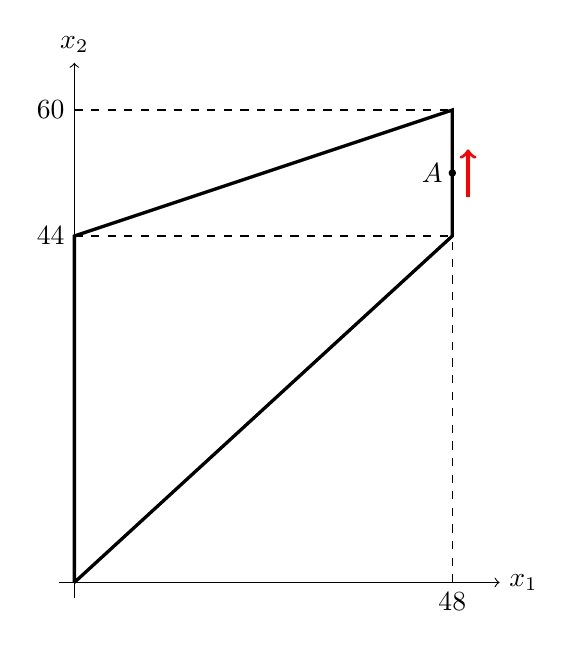
\begin{tikzpicture}[scale=0.1]
\draw[-,very thick] (0,0) -- (48,44) -- (48,60) -- (0,44) -- (0,0);
\node[left] at (0,44) {$44$};
\node[left] at (0,60) {$60$};
\node[below] at (48,0) {$48$};
\draw[->] (-2,0) -- (54,0);
\node[right] at (54,0) {$x_1$};
\draw[->] (0,-2) -- (0,66);
\node[above] at (0,66) {$x_2$};
\draw[dashed] (0,44) -- (48,44);
\draw[dashed] (0,60) -- (48,60);
\draw[dashed] (48,0) -- (48,44);
\node[left] at (48,52) {$A$};
\draw[fill](48,52) circle (0.4);
\draw[->,very thick,red] (50,49) -- (50,55);
\end{tikzpicture}
\end{center}
\end{document}
